\section{Introduction}


\subsection{What is a decision tree?} \label{whatisadecisiontree}
An economy student with only a very few programming skills shall develop a simple algorithm for sorting three elements $A, B, C$. He decides to divide this problem in smaller subproblems. First he wonders if $A$ is smaller than $B$. In the second step it is interesting if $B$ is smaller than $C$. If $A<B$ and $B<C$ than $A<B<C$. But if $B$ is not greater than $C$, than a third question is relevant: Is $A<C$? 

His head is spinning. Maybe solving this problem graphically is a better idea. He draws a node for each question and an edge for each answer. All leafs represent the correct order. Figure \ref{fig:sortingtree} shows the resulting graph:

\begin{figure}[!h]
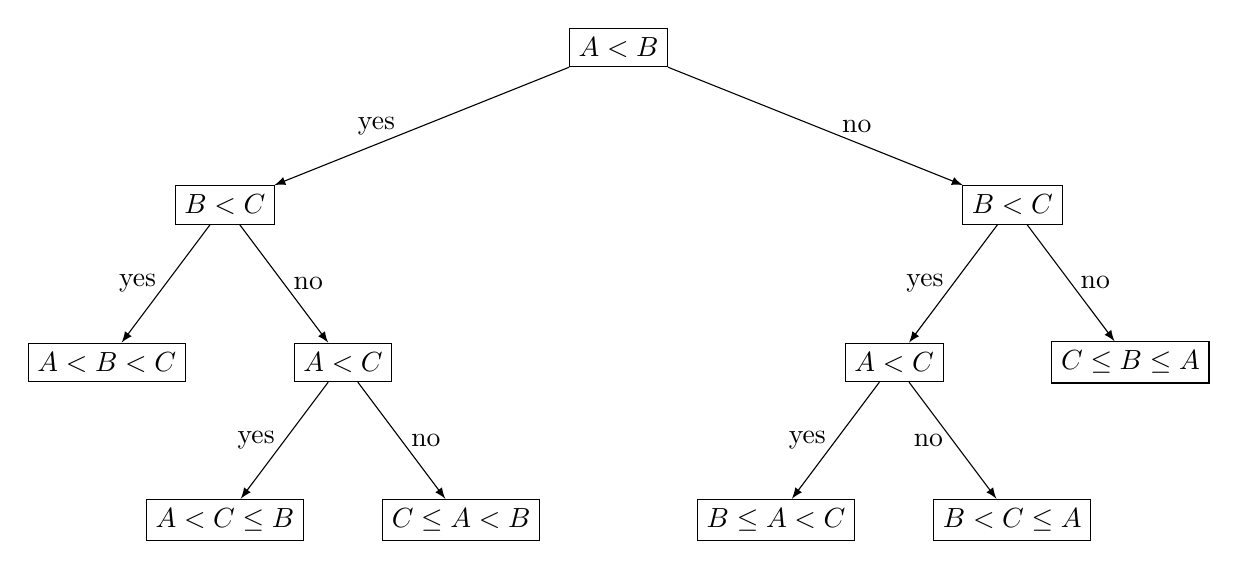
\begin{tikzpicture}[edge from parent/.style={draw,-latex},
level distance=2cm,
level 1/.style={sibling distance=10cm},
level 2/.style={sibling distance=3cm}]
\tikzstyle{every node}=[rectangle,draw]    
\node (Root) {$A < B$}
child {
    node {$B < C$}    
    child { 
        node {$A < B < C$} 
        edge from parent node[left,draw=none] {yes}
    }
    child { 
        node {$A < C$} 
        child {
            node {$A < C \leq B$}
            edge from parent node[left,draw=none] {yes}
        }
        child {
            node {$C \leq A < B$}
            edge from parent node[right,draw=none] {no}
        }
        edge from parent node[right,draw=none] {no}
    }
    edge from parent node[left,draw=none] {yes $\;$}
}
child {
    node {$B < C$}
    child { 
        node {$A < C$}     
        child {
            node {$B \leq A < C$}
            edge from parent node[left,draw=none] {yes}
        }   
        child {
            node {$B < C \leq A$}
            edge from parent node[left,draw=none] {no}
        }     
        edge from parent node[left,draw=none] {yes}
    }
    child { 
        node {$C \leq B \leq A$} 
        edge from parent node[right,draw=none] {no}
    }
    edge from parent node[right,draw=none] { $\;$ no}
};
\end{tikzpicture}
\caption{A decision tree for sorting three values.}
\label{fig:sortingtree}
\end{figure}

Without further knowledge the student created his first decision tree.

For a right decision two or three if-statements are necessary. So a Python program could look like listing \ref{lst:sort1}.

\newpage

\begin{lstlisting}[style = siemens, language = Python, caption={[A Python implementation of a decision tree for sorting three elements]A Python implementation of a decision tree for sorting three elements $A, B, C$},label=lst:sort1]
def sort1(A, B, C):
	if (A < B):
		if (B < C):
			return [A, B, C]
		else:
			if (A < C):
				return [A, C, B]
			else:
				return [C, A, B]
	else:
		if (B < C):
			if (A < C):
				return [B, A, C]
			else:
				return [B, C, A]
		else:
			return [C, B, A]

print( sort1(9,-2,0) ) # >> [-2, 0, 9]
print( sort1(2,0,0) )  # >> [0, 0, 2]
\end{lstlisting}

\begin{remark}
    The Python if-statement syntax and intends implies the tree structure in a vertical form, too.      
\end{remark}

Another way of formatting if-clauses represents a rule set which are first order logical expressions:  
    \begin{lstlisting}[style = siemens, language = Python, caption={A Python reimplementation of the decision tree given in listing \ref{lst:sort1} as a set of first order logical rules},label=lst:sort2]
def sort2(A, B, C):
	if (A < B) and (B < C) : return [A, B, C]
	if (A < B) and not (B < C) and (A < C): return [A, C, B]
	if (A < B) and not (B < C) and not (A < C): return [C, A, B]
	if not (A < B) and (B < C) and (A < C): return [B, A, C]
	if not (A < B) and (B < C) and not (A < C): return [B, C, A]
	if not (A < B) and not (B < C) : return [C, B, A]
\end{lstlisting}

Unsurprisingly, we get six rules for $3! = 6$ different combinations and the same results as in the algorithm \texttt{sort1}. 


This introductory example shows four main things: Decision trees
\begin{enumerate}
    \item work very well for classification and data mining.
    \item are intuitive and self-explanatory.
    \item They are easy to implement.
    \item can be even used by economists.
\end{enumerate}

\begin{remark}
    Decision trees are used to model all comparison sorts like mergesort or quicksort. The reader may notice that the decision tree in figure \ref{fig:sortingtree} represents the insertion sort algorithm \cite[p. 208]{cormen2001introduction}. 
\end{remark}




\subsection{Taxonomy}\label{taxonomy}

Before we approach the theory behind decision trees, a small but general overview of the taxonomy shall be given.

Decision tree classification is very often used in the context of data mining and machine learning. These keywords are no synonyms -- although used as one very often. Machine learning cannot be seen as a true subset of data mining, as it also contains other fields, not utilized for data mining (e.g. theory of learning, computational learning theory, and reinforcement learning).

Figure \ref{fig:machinelearningcontext} shows the machine learning context for decision trees. 

\begin{figure}[!h] \centering
\begin{tikzpicture}[
edge from parent path={(\tikzparentnode\tikzparentanchor) -- (\tikzchildnode.north)},
every node/.style={text centered, draw=none, anchor=north, draw=none, fill=white, minimum height=1.5em},
%level distance=1.5cm,
level 1/.style={sibling distance=3.5cm, level distance=1cm},
level 2/.style={sibling distance=3.5cm, level distance=2cm}]
\node (Root) {Machine Learning Algorithms} 
child { 
    node [draw, dashed, text width=7em] {Unsupervised Learning}
    child[grow=south west] {node {\dots}}
}
child { 
    node [draw, dashed, text width=13em, yshift=-1.5cm] {
        \begin{tikzpicture}[level 2/.style={sibling distance=2.7cm, level distance=0.75cm}] 
            \node[text width=12em, text=siemensblue] {Supervised Learning } 
            child [] {
                node [text width=6em, text=siemensblue] {Classification}
                edge from parent[draw, solid]
            }
            child {
                node[text width=5em] {Regression}
                edge from parent[draw, solid]
            };
        \end{tikzpicture}
    } % end node
    child[] {
        node[text=siemensblue] {Decision Tree}
    }    
    child[] {
        node[text width=7em] {Artificial Neural Network}
    }
    child[] {
        node[text width=7em] {Support Vector Machines}
    }    
    child[] {
        node {\dots}
    }
}
child { 
    node[draw, dashed, text width=7em] {Reinforcement Learning}
    child[grow=south east] {node {\dots}}
}
child { 
    node[draw, dashed, text width=7em] {Deep Learning}
    child[grow=south east] {node {\dots}}
}
;
\end{tikzpicture}
\caption[The context of decision trees in machine learning with in this paper visited topics.]{The context of decision trees in machine learning with \textcolor{siemensblue}{in this paper visited topics}.}
\label{fig:machinelearningcontext}
\end{figure}

\begin{remark}
The context shown in figure \ref{fig:machinelearningcontext} is not intended for being complete, e.g. there is mixture of unsupervised and supervised learning, so called semi-supervised learning. Also not every decision tree can handle continuos values for regression analysis as we will see later.
\end{remark}

Decision trees have a sibling, called regression trees. They have a common parent: prediction trees \cite{goldman2010self}. The basic idea is to use trees to model functions though each end point will result in the same predicted value, a constant for that point. Thus a regression tree is like a classification tree except that the end point will be a predicted function value rather than a predicted classification. 


%\begin{figure}[!h] \centering
%\begin{tikzpicture}[edge from parent/.style={draw, open triangle 60-},
%level distance=1.5cm,
%level 1/.style={sibling distance=1cm},
%level 2/.style={sibling distance=4cm}]
%\tikzstyle{every node}=[rectangle,draw]    
%\node (Root) {Tree}
%child { 
%    node {Prediction Tree}
%    child{ node{Classification Tree} }
%    child{ node{Regression Tree} }
%};
%\end{tikzpicture}
%\caption{An UML-like pedigree of classification and regression trees. }
%\label{fig:predictiontree}
%\end{figure}
   
Although, there is a wide field of applications for regression trees, the focus of this paper in only on classification trees.



\subsection{About this paper}

This project work emerges in the context of the course \textit{Artificial Intelligence} in the winter semester 2013/2014. Beside this seminar paper, an introductory presentation was conducted and an implementation for decision tree was developed. 

In the scope of this seminar paper, a small introduction to theory and application of decision trees shall be given. 

After this short introduction a theoretical consideration shall guide to a practical part, which shall clarify the theoretical part by examples. The last part shall summarize and compare the introduced algorithm and shall give a small outlook to not tackled research fields of decision trees.

On the contrary to the presentation during the seminar, this seminar paper expects a basic knowledge about graph theory, complexity, and machine learning. Instead of an introduction to these underlaying topics, a deeper look inside four decision tree algorithm families shall be given: \textsc{CHAID}, \textsc{CART}, \textsc{ID3}, and \textsc{C4.5}.  

The focus of all Python implementation is on classification. This limitation is not owed to the insufficient importance of regression calculating, but a wider look would push the boundaries of this seminar paper.   

\begin{remark}
    Remark boxes like this one shall help to see the bigger pictures. It contains information that will not be explained any further, but which are a starting point for further investigations.
\end{remark}




\newpage
